\documentclass[11pt,a4paper,titlepage]{report}
\usepackage[T1]{fontenc}
\usepackage[utf8]{inputenc}
\usepackage[french]{babel}
\usepackage{lmodern}
\usepackage{geometry}
\usepackage{xcolor}
\usepackage{graphicx}
\usepackage{hyperref}
\usepackage{booktabs}
\usepackage{fancyhdr}
\usepackage{listings}
\usepackage{enumitem}
\usepackage{amsmath}

\geometry{top=2.5cm, bottom=2.5cm, left=2.5cm, right=2.5cm}

\definecolor{primary}{RGB}{15, 23, 42}
\definecolor{accent}{RGB}{245, 158, 11}
\definecolor{secondary}{RGB}{16, 185, 129}
\definecolor{darkgray}{RGB}{51, 65, 85}
\definecolor{lightgray}{RGB}{241, 245, 249}

\hypersetup{
    colorlinks=true,
    linkcolor=primary,
    filecolor=primary,      
    urlcolor=accent,
    citecolor=secondary,
    pdfauthor={Malick Buss Engineering},
    pdftitle={Malick Buss - Dossier d'Architecture et Manuel d'Exploitation Enterprise}
}

\pagestyle{fancy}
\fancyhf{}
\fancyhead[L]{\textcolor{darkgray}{\textbf{Malick Buss} — Dossier d'Architecture Technique}}
\fancyhead[R]{\textcolor{darkgray}{Version 1.0.0}}
\fancyfoot[L]{\textcolor{darkgray}{Confidentiel — Usage Interne}}
\fancyfoot[R]{\thepage}
\renewcommand{\headrulewidth}{0.4pt}
\renewcommand{\footrulewidth}{0.4pt}

\lstset{
    backgroundcolor=\color{lightgray},
    basicstyle=\ttfamily\footnotesize,
    breaklines=true,
    captionpos=b,
    frame=single,
    rulecolor=\color{darkgray},
    numbers=left,
    numberstyle=\tiny\color{darkgray},
    showstringspaces=false
}

\begin{document}

\begin{titlepage}
    \centering
    \vspace*{1.5cm}
    
    {\Huge \bfseries \textcolor{primary}{MALICK BUSS SÉNÉGAL}}\\[0.5cm]
    {\LARGE \textcolor{accent}{\textbf{Marketplace E-Commerce Multi-Boutiques}}}\\[1.5cm]
    
    \rule{\linewidth}{1.5pt}\\[0.4cm]
    {\huge \bfseries Dossier d'Architecture Technique, Spécifications Opérationnelles \& Guide de Déploiement Hybride}\\[0.2cm]
    \rule{\linewidth}{1.5pt}\\[2cm]
    
    \begin{minipage}{0.45\textwidth}
        \begin{flushleft} \large
            \textbf{Auteurs :}\\
            Équipe Ingénierie \& DevOps\\
            Malick Buss Tech Core
        \end{flushleft}
    \end{minipage}
    \begin{minipage}{0.45\textwidth}
        \begin{flushright} \large
            \textbf{Statut :} Production Ready\\
            \textbf{Version :} 1.0.0\\
            \textbf{Date :} \today
        \end{flushright}
    \end{minipage}
    
    \vfill
    
    {\large \textbf{Plateforme Mobile-First • Transactions FCFA (Wave / Orange Money) • CI/CD \& SonarQube}}\\[0.5cm]
    {\small Dakar, République du Sénégal}
\end{titlepage}

\tableofcontents
\newpage

\chapter{Contexte Stratégique \& Vision Produit}

\section{Vision Globale \& Piliers Fondamentaux}
\textbf{Malick Buss} est une marketplace multi-boutiques mobile-first conçue spécifiquement pour répondre aux exigences structurelles du commerce digital au Sénégal (Dakar et régions de l'intérieur) et dans l'UEMOA.

La plateforme articule sa proposition de valeur autour de 4 piliers fondamentaux :
\begin{enumerate}[label=\textbf{\arabic*.}]
    \item \textbf{Garantie de Confiance \& Authenticité Produits :} Éradication de la contrefaçon et des photos trompeuses grâce à l'obligation de capture vidéo et photo en direct (\textit{Direct Camera Live Capture}).
    \item \textbf{Étanchéité Financière \& Traçabilité :} Calcul automatique et transparent d'une commission marketplace de 10\% par vente validée, avec isolation stricte des sous-commandes et journalisation comptable inviolable (\textit{Commission Ledger}).
    \item \textbf{Intégrations Locales en FCFA :} Support natif des solutions de paiement plébiscitées (Wave, Orange Money) et encadrement strict du Paiement à la Livraison (\textit{Cash On Delivery}).
    \item \textbf{Synergie WhatsApp Sécurisée :} Exploitation de WhatsApp pour la réassurance et l'assistance client, sans compromission des flux financiers de la marketplace.
\end{enumerate}

\section{Acteurs \& Modèle des Rôles (RBAC)}
\begin{itemize}
    \item \textbf{Acheteur (CLIENT) :} Recherche géolocalisée, constitution d'un panier multi-boutiques unique, suivi d'expédition temps réel et réclamations sous 7 jours.
    \item \textbf{Vendeur / Marchand (VENDOR) :} Gestion autonome de la boutique, publication d'articles certifiés, traitement d'états des commandes et demande de retrait de solde vers Wave/Orange Money.
    \item \textbf{Super Administrateur (SUPER\_ADMIN) :} Pouvoirs de gouvernance régalienne, modération de catalogue, vérification KYC des marchands, arbitrage des litiges et exécution des décaissements financiers.
\end{itemize}

\chapter{Architecture Logicielle \& Modèle de Données}

\section{Organisation du Monorepo}
Le projet est architecturé sous la forme d'un monorepo modulaire garantissant la réutilisabilité du code et le typage strict de bout en bout :
\begin{itemize}
    \item \textbf{\texttt{shared/}} : Bibliothèque partagée de types TypeScript, DTOs communs, utilitaires monétaires (\texttt{formatFCFA}) et formatage téléphonique international (\texttt{formatPhoneForWhatsApp}).
    \item \textbf{\texttt{backend/}} : API REST Core développée avec NestJS, validation DTO, authentification JWT, ORM Prisma et persistance PostgreSQL 16.
    \item \textbf{\texttt{frontend/}} : Application Web client et portail marchand développée en Next.js 14 App Router, optimisée pour les connexions mobiles 3G/4G.
    \item \textbf{\texttt{back-office/}} : Console de supervision et d'administration Super Admin (Next.js 14, Tailwind CSS, tableaux de bord de modération et gouvernance).
\end{itemize}

\section{Modèle de Données Relationnel (PostgreSQL \& Prisma)}
La base de données relationnelle est orchestrée autour d'un schéma robuste :
\begin{itemize}
    \item \textbf{Utilisateurs \& Sécurité :} \texttt{users}, \texttt{roles}, \texttt{refresh\_tokens}, \texttt{audit\_logs}.
    \item \textbf{Boutiques \& KYC :} \texttt{shops} avec statuts (\texttt{PENDING\_VERIFICATION}, \texttt{ACTIVE}, \texttt{SUSPENDED}, \texttt{REJECTED}), coordonnées certifiées et toggle \texttt{requireLiveCapture}.
    \item \textbf{Catalogue Produits :} \texttt{products} avec gestion de stock, prix de base, prix remisé, conditions (\texttt{NEUF}, \texttt{TRES\_BON\_ETAT}) et URLs Cloudinary.
    \item \textbf{Commandes \& Sous-Commandes :} \texttt{orders} parentes éclatées en \texttt{sub\_orders} par marchand, permettant des cycles de vie indépendants (\texttt{PENDING\_PAYMENT}, \texttt{TO\_ACCEPT}, \texttt{ACCEPTED}, \texttt{PREPARING}, \texttt{SHIPPED}, \texttt{DELIVERED}, \texttt{COMPLETED}).
    \item \textbf{Grand Livre Financier :} \texttt{commission\_ledgers} et \texttt{withdrawal\_requests} pour la comptabilisation irréversible des gains et décaissements.
\end{itemize}

\chapter{Cartographie des Use Cases du Super Admin}

\section{Synthèse des 8 Domaines Opérationnels}
\begin{table}[h!]
\centering
\small
\begin{tabular}{@{}llp{8.5cm}@{}}
\toprule
\textbf{Domaine} & \textbf{Désignation} & \textbf{Responsabilités \& Actions Clés} \\
\midrule
\textbf{Domaine 1} & Pilotage \& KPI & Chiffre d'affaires global, volume des transactions, commissions perçues. \\
\textbf{Domaine 2} & Onboarding \& KYC & Validation des dossiers marchands, activation et politique caméra directe. \\
\textbf{Domaine 3} & Relations Vendeurs & Annuaire unifié, contact direct WhatsApp wa.me/221..., suspension/réactivation. \\
\textbf{Domaine 4} & Modération Catalogue & Dépublication des articles non conformes, vérification anti-contrefaçon. \\
\textbf{Domaine 5} & Supervision Commandes & Suivi des sous-commandes, arbitrage des réclamations clients, remboursements. \\
\textbf{Domaine 6} & Gestion Financière & Validation des retraits marchands (seuil 5 000 FCFA), audit des virements Wave/OM. \\
\textbf{Domaine 7} & Sécurité \& RBAC & Gestion des privilèges, désactivation de comptes suspects, journal d'audit. \\
\textbf{Domaine 8} & Gouvernance & Paramétrage du taux de commission (10\%), frais de livraison (3 000 FCFA). \\
\bottomrule
\end{tabular}
\caption{Matrice des responsabilités opérationnelles du Super Administrateur}
\end{table}

\chapter{Sécurité, Qualité de Code \& SonarQube}

\section{Mesures de Sécurité Avancées}
\begin{itemize}
    \item \textbf{Chiffrement des Mots de Passe :} Dérivation de clé cryptographique via l'algorithme \texttt{scrypt} avec sel cryptographique de 16 octets et comparaison en temps constant (\texttt{timingSafeEqual}) pour prévenir les attaques temporelles.
    \item \textbf{En-têtes HTTP de Sécurité :} Injection systématique des en-têtes \texttt{X-Content-Type-Options: nosniff}, \texttt{X-Frame-Options: SAMEORIGIN}, \texttt{Referrer-Policy: strict-origin-when-cross-origin} et suppression de l'en-tête discriminant \texttt{X-Powered-By}.
    \item \textbf{Protection CORS Dynamique :} Filtrage strict des requêtes cross-origin avec support automatique des domaines de preview et de production Vercel (\texttt{*.vercel.app}) et des domaines officiels Malick Buss.
\end{itemize}

\section{Contrôle Qualité \& SonarQube Quality Gate}
Le fichier de configuration \texttt{sonar-project.properties} assure une couverture complète :
\begin{lstlisting}[language=bash, caption=Configuration SonarQube de l'entreprise]
sonar.projectKey=malick-buss
sonar.projectName=Malick Buss Marketplace
sonar.sources=backend/src,frontend/src,back-office/src,shared/src
sonar.tests=backend/test
sonar.javascript.lcov.reportPaths=backend/coverage/lcov.info
\end{lstlisting}

\begin{figure}[h!]
\centering
\IfFileExists{assets/architecture/architecture-cloud-cicd.jpg}{
    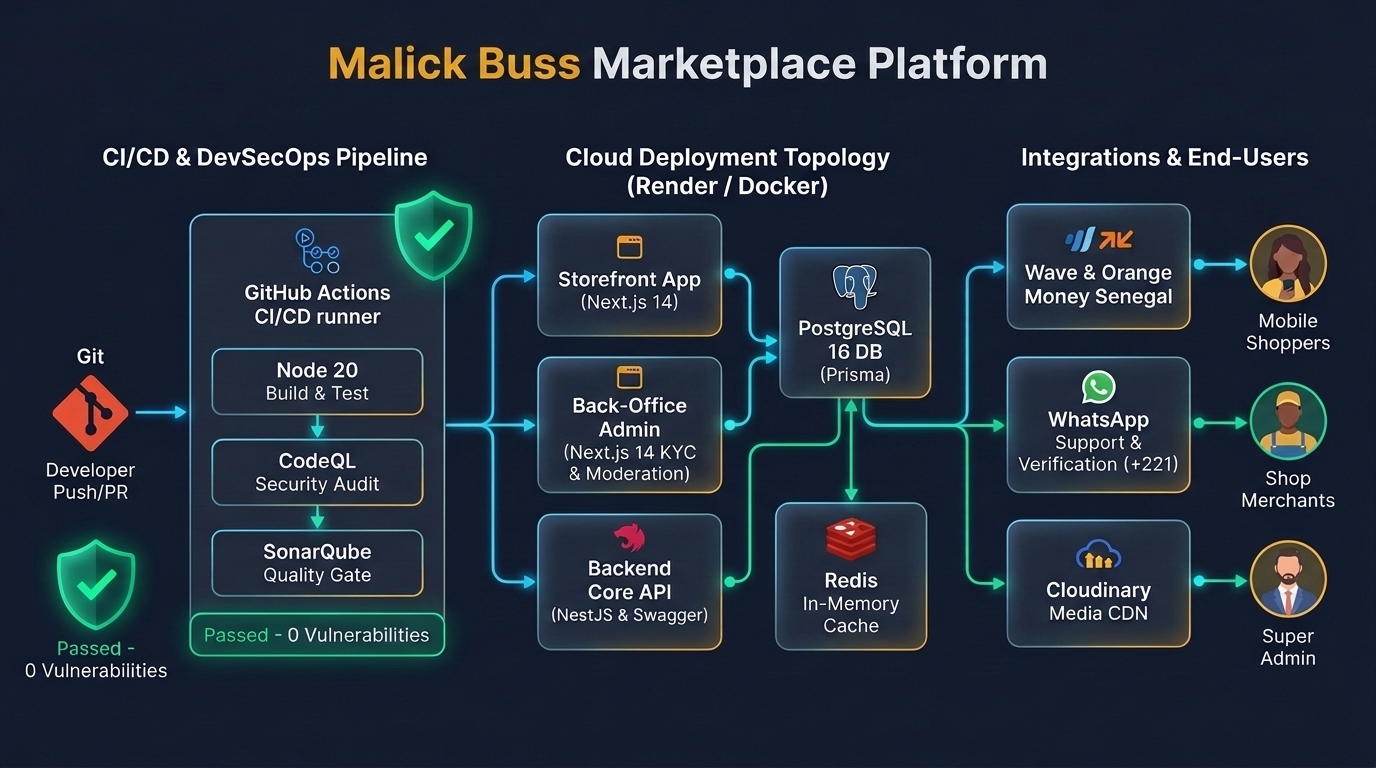
\includegraphics[width=0.92\linewidth]{assets/architecture/architecture-cloud-cicd.jpg}
}{
    \fbox{Illustration architecture-cloud-cicd.jpg}
}
\caption{Architecture Globale Cloud, CI/CD et Quality Gate SonarQube}
\end{figure}

\chapter{DevOps, Déploiement Hybride \& CI/CD}

\section{Stratégie Hybride : Render \& Vercel}
L'architecture de production dissocie la charge de travail pour une résilience maximale :
\begin{itemize}
    \item \textbf{Render (Backend Core) :} Hébergement du service API NestJS et de la base managée PostgreSQL 16. La commande de pré-déploiement exécute automatiquement \texttt{npx prisma migrate deploy}.
    \item \textbf{Vercel (Frontends Edge) :} Déploiement de l'application cliente et de la console d'administration sur le réseau mondial Vercel Edge avec purge de cache instantanée.
\end{itemize}

\begin{figure}[h!]
\centering
\IfFileExists{assets/architecture/schema-structurel-flux-operationnel.jpg}{
    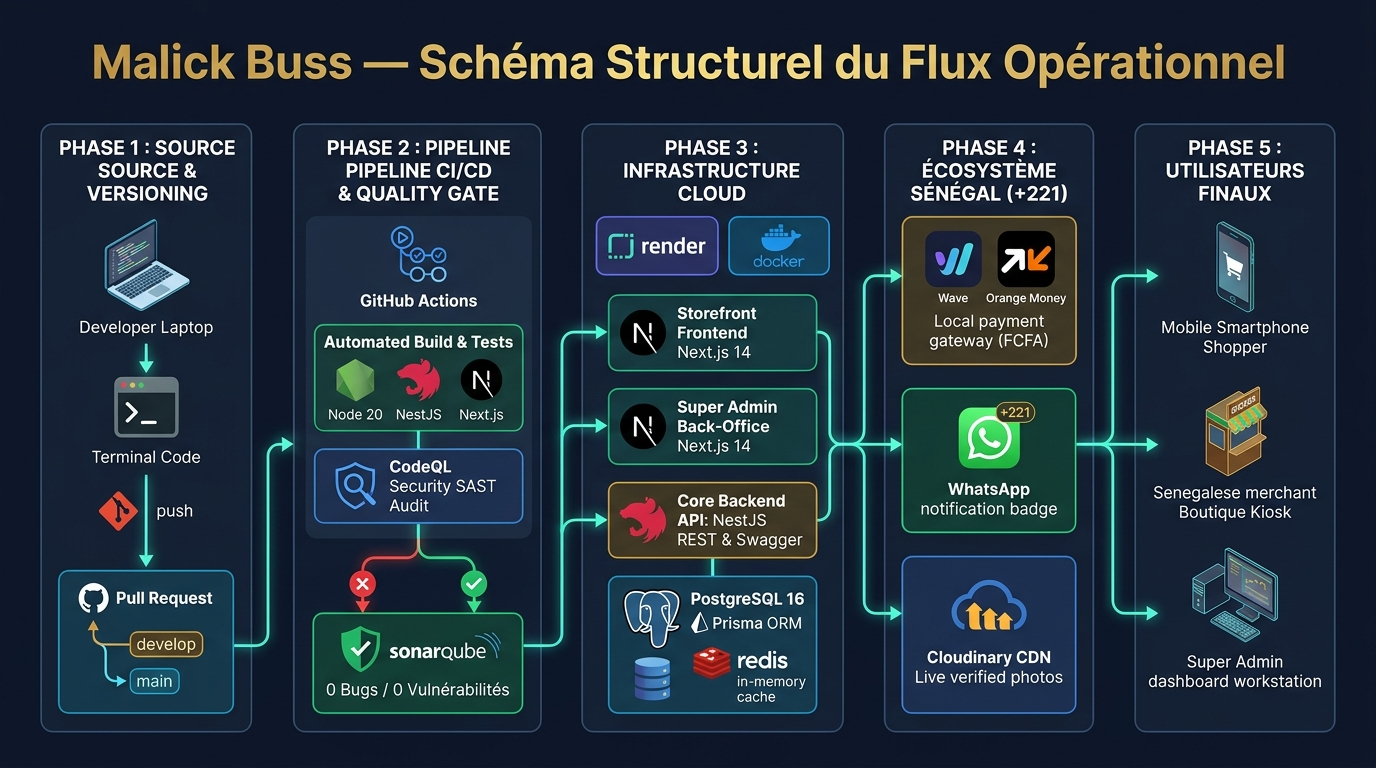
\includegraphics[width=0.92\linewidth]{assets/architecture/schema-structurel-flux-operationnel.jpg}
}{
    \fbox{Illustration schema-structurel-flux-operationnel.jpg}
}
\caption{Schéma Structurel du Flux Opérationnel en 5 Phases}
\end{figure}

\section{Sondes de Santé HTTP}
L'API expose deux points de contrôle cruciaux pour les orchestrateurs cloud :
\begin{itemize}
    \item \texttt{GET /health/live} : Vérifie que le processus Node.js est actif et traite les requêtes.
    \item \texttt{GET /health/ready} : Exécute une requête \texttt{SELECT 1} sur PostgreSQL pour confirmer la disponibilité de la couche de données avant d'orienter le trafic client.
\end{itemize}

\chapter{Conclusion \& Manuel d'Exploitation}

\section{Commandes Usuelles pour l'Équipe}
\begin{table}[h!]
\centering
\small
\begin{tabular}{@{}ll@{}}
\toprule
\textbf{Commande npm} & \textbf{Effet / Action Opérationnelle} \\
\midrule
\texttt{npm run build:shared} & Compilation de la librairie partagée TypeScript. \\
\texttt{npm run build:backend} & Compilation NestJS de l'API de production. \\
\texttt{npm run build:frontend} & Génération statique des 42 pages de la vitrine client. \\
\texttt{npm run build:admin} & Génération statique de la console Super Admin. \\
\texttt{npm run test --workspace=backend} & Exécution des 8 tests unitaires de logique financière. \\
\texttt{npm run test:api --workspace=backend} & Exécution des 4 suites de tests d'intégration API. \\
\texttt{npm run test:coverage} & Génération du rapport de couverture LCOV pour SonarQube. \\
\texttt{npm run sonar:up} & Démarrage du serveur SonarQube Community en local via Docker. \\
\texttt{npm run doc:build} & Compilation du présent rapport technique en PDF haute fidélité. \\
\bottomrule
\end{tabular}
\caption{Répertoire des commandes opérationnelles du projet}
\end{table}

\vfill
\begin{center}
    \small \textcolor{darkgray}{Document validé conforme par l'équipe d'architecture Malick Buss — Tous droits réservés © 2026.}
\end{center}

\end{document}
